% Chapter 3

\chapter{Data Exploration} % Main chapter title

Before discussing the methods it is useful to first ground ourselves in the data. Here we provide some preliminary analysis that was performed that helped shape the design decisions in the next chapter.

\label{Chapter3}

\subsection{Daily play patterns}

Track plays by hour of the day demonstrate a clear daily pattern with usage hitting the peak at around 5pm and a trough at around 6am. 

\begin{figure}[h!]
	\centering
	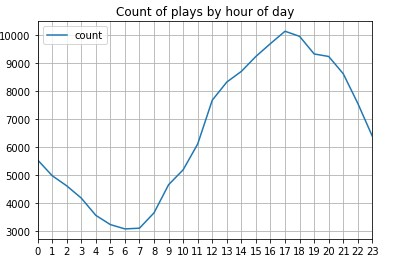
\includegraphics[width=7cm, keepaspectratio,]{fig004.jpg}
	\caption{5-5.30pm is peak listening time}
	\label{fig:fig4}
\end{figure} 

The peak of 5pm is easily explained by 9-5 workers finishing their jobs, however decline during pre-work hours of 6-8am was unexpected and may be a product of how the data was gathered.

Zooming out to view the pattern across an entire week we see that the daily pattern is occurs across every day of the week

\begin{figure}[h!]
	\centering
	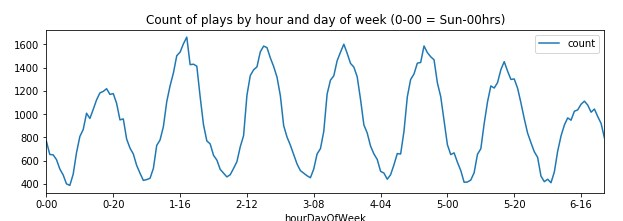
\includegraphics[width=7cm, keepaspectratio,]{fig005.jpg}
	\caption{Most popular times to listen to music across all users}
	\label{fig:fig5}
\end{figure} 


A sample of users also showed 

\begin{figure}[h!]
	\centering
	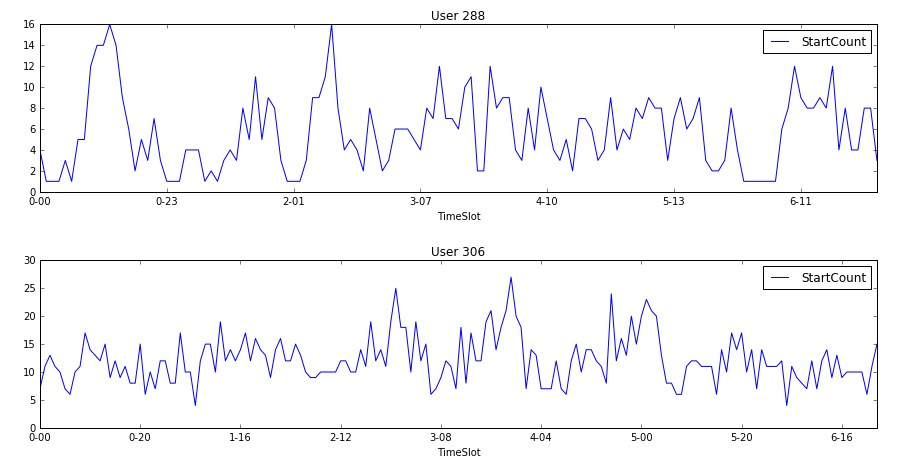
\includegraphics[width=7cm, keepaspectratio,]{fig006.jpg}
	\caption{Most popular times to listen to music by individual user}
	\label{fig:fig6}
\end{figure} 

\subsection{Inter-event times}

The dataset contains a timestamp associated with each user. This does not necessarily mean the user played a song in its entirety. Analysis shows plenty of cases where the interval time between tracs was a few seconds suggesting the user skipped tracks.

\begin{figure}[h!]
	\centering
	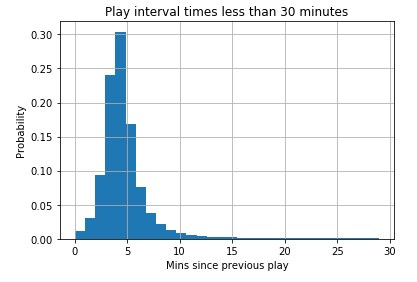
\includegraphics[width=7cm, keepaspectratio,]{fig003.jpg}
	\caption{}
	\label{fig:fig3}
\end{figure} 

However for our purposes we can include these as evidence that the user was interested in playing music at time $t$.

We can also assume that the song plays are not i.i.d, in that the probability of a play event at time t+1 is significantly higher if there was an event at time t. 

\subsection{Outlier analysis}

An analysis of plays by user reveals a high amount of variance between users on how many tracks are played. 
\begin{figure}[h!]
	\centering
	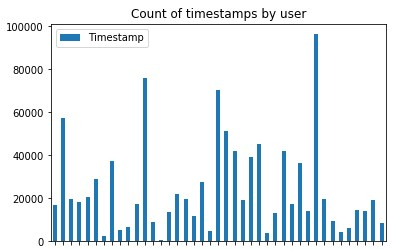
\includegraphics[width=7cm, keepaspectratio,]{fig002.jpg}
	\caption{}
	\label{fig:fig2}
\end{figure} 

\subsection{Conclusion}